\chapter{Supervised Progressive Autonomous Robot \newline Competencies}\label{chap:sparc}
\glsresetall
\graphicspath{{images/sparc/}}

\begin{framed}
	\textbf{Key points:}
	%CHeck for 
	\begin{itemize}
		\item Proposition of a novel interaction framework to teach robots an action policy while interacting.
		\item A human teacher is in control of the robot's actions whilst the robot learns from this supervision.
		\item The teacher can select actions to be executed by the robot.
		\item The robot proposes actions about to be executed to the teacher.
		\item The teacher provides feedback on propositions (i.e. intentions) rather than executed actions; and can preempt actions.
		\item The robot's behaviour (under supervision) can be assumed to be optimal.
		\item The workload on the teacher decreases over time as the robot learns.
	\end{itemize}
\end{framed}

Parts of the work presented in this chapter have been published in \cite{senft2015sparc} and \cite{senft2017supervised}. The final publications are available from Springer and Elsevier:
\begin{itemize}
	\item \url{http://dx.doi.org/10.1007/978-3-319-25554-5_60}.
	\item \url{https://doi.org/10.1016/j.patrec.2017.03.015}.
\end{itemize}

\newpage
\section{Motivation}
As presented in Chapter~\ref{chap:background}, robots would profit from being able to learn from human teachers how to interact with other humans. We propose to use \gls{iml} to achieve this transfer of social and task knowledge from the human domain-expert to the robot. This would result in a faster and safer learning than slow iterative update of behaviours by engineering the action policy, learning from large quantities of data or learning by trials and errors as with \gls{rl}.

However, as stated in this Section~\ref{sec:back_iml}, \gls{iml} has never been applied to teach robots to interact with humans. No current system provides the teacher with enough control over the robot's actions to validate the first principle presented in Section~\ref{ssec:back_constraints} (`Only execute appropriate actions'). Techniques relying solely on feedback from the teacher cannot prevent the robot to execute an incorrect action, but only reduce the chances of future errors by rewarding negatively incorrect actions after their execution~\citep{senft2017supervised}. And, with current techniques based on \gls{lfd} the teacher relinquishes its control over the robot when not demonstrating, only reacting in hindsight after the learner makes mistakes and its erroneous actions have impacted the real world~\citep{chernova2009interactive}.

The problem tackled in this research is to provide a robot with an appropriate action policy, adaptive to different contexts and partners' behaviours and requiring a low workload on the teacher. As such, in \cite{senft2015sparc}, we introduced the \gls{sparc} framework of interaction. \gls{sparc} aims to allow end-users to safely and easily teach a robot an action policy applicable to social \gls{hri}.

%Whilst \gls{sparc} has been developed to allow robots to learn how to interact socially with humans, it could also be applied to any type of agent learning to interact in an environment. Similarly, the terms `supervisor' and `teacher' are exchangeable as the teacher teaches the robot how to behave while supervising its behaviour.

\section{Frame}

Similarly to other applications of \gls{iml}, \gls{sparc} requires inputs from a teacher to learn an action policy to interact with the world. As framed in the introduction, in this framework, the robot interacts with two entities: the target and the teacher (as shown in Figure~\ref{fig:frame}). This results into two intertwined interactions: the application interaction (task the robot learns to achieve) and the teaching interaction (relation with the teacher). In the generic case, the overall interaction is a triadic interaction (Teacher - Robot - Human target or Teacher - Robot - Environment); for instance, a teacher could teach a tutor robot to support child learning in an education task (as implemented in Chapter~\ref{chap:tutoring}). But in specific cases, the application target is not a human but only part of the environment, such as a robot at home learning from its user how to support them better.

\begin{figure}[ht]
	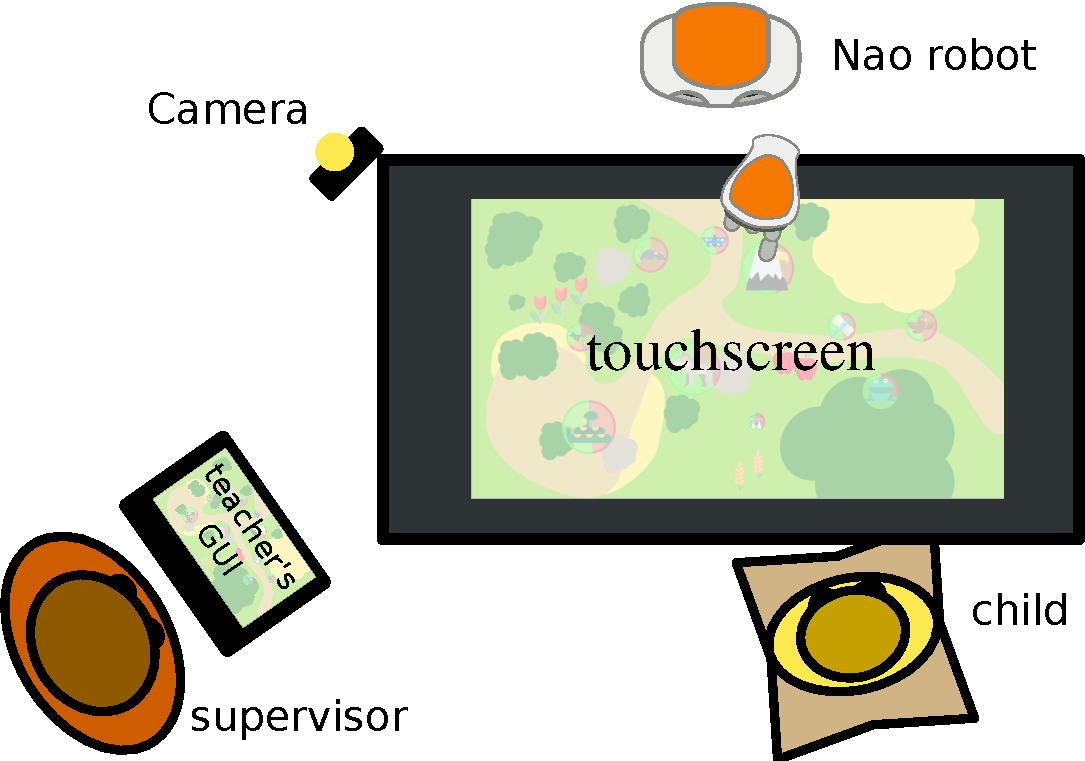
\includegraphics[width=.6\linewidth]{setup.pdf}
	\centering
	\caption{Frame of the interaction: a robot interacts with a target, suggests actions and receive commands and feedback from a teacher. Using machine learning, the robot improves its suggestions over time, to reach an appropriate action policy.}
	\label{fig:frame}
\end{figure}

\section{Principles} \label{sec:sparc_principles}

\gls{sparc} defines an interaction between a learner (virtual agent or robot) and a teacher following these principles:
\begin{itemize}
	\item The learner has access to a representation of the state of the world and a set of actions.
	\item The teacher can select actions for the robot to execute.
	\item The learner can propose actions to the teacher before executing them (informing them about its intentions).
	\item The teacher can enforce or cancel actions proposed by the learner and actions non evaluated are implicitly validated and executed after a short delay.
	\item The learner uses \gls{ml} to improve its action policy using the teacher's commands and feedback on propositions.
\end{itemize} 

This type of interaction between the learner and the teacher is similar to the level 6 on the Sheridan scale of autonomy: "computer selects action, informs human in plenty of time to stop it"~\citep{sheridan1978human}; with the addition that the human has also the opportunity to select actions for the agent to execute. In this thesis, we will refer to this interaction as `\gls{sa}': the robot interacts autonomously under the supervision of a human who can ensure that the robot's behaviour is constantly appropriate.

This way of keeping a human in the learning loop, with the opportunity to override the agent actions, and the robot learning from these demonstrations is similar to Dogged Learning~\citep{grollman2007dogged}. However, with \gls{sparc}, this ability to provide demonstrations is combined with the \gls{sa}. This results in a mixed control system where the teacher can select actions and have the robot execute them while the robot only proposes actions to the teacher. In response to this suggestion, the teacher has the choice between preempting the action or let it be executed. A learning algorithm on the robot's side uses the feedback and commands from the teacher to improve the correctness of the suggested actions until reaching an efficient action policy. This learning mechanism coupled with auto-execution of actions aims to decrease the requirement of interventions from the teacher over time, thus reducing the workload on the teacher as the robot learns. Additionally, keeping the human in the loop also gives them the opportunity to provide additional information to the algorithm speeding up the learning and to create a mental model of the learner. The diagram in Figure~\ref{fig:sparc_diagram} and the flowchart in Figure~\ref{fig:sparc_flowchart} represent in a graphical way this interaction between the learner and the teacher.

\begin{figure}[ht]
	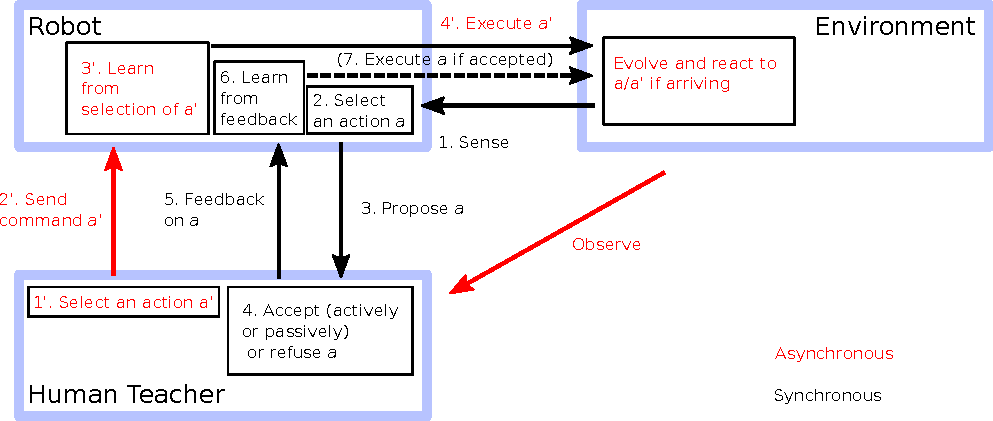
\includegraphics[width=1\linewidth]{diagram.pdf}
	\centering
	\caption{Diagram of interaction between the robot, the human teacher and the environment with \gls{sparc}: synchronously, the robot can propose actions to the teacher that evaluated (approved or cancelled). And asynchronously, the teacher can select actions to be executed.}
	\label{fig:sparc_diagram}
\end{figure}

Additionally, The main difference between \gls{sparc} and CBA~\citep{chernova2009interactive} is that with \gls{sparc}, the robot communicates its intentions and the teacher has total control over the robot's action. With CBA and other classical \gls{iml}, the teacher have to wait for an action to impact the world before correcting it or assigning it a negative feedback~\citep{thomaz2008teachable,knox2009interactively}. However, using \gls{sparc}, the teacher is informed beforehand of the robot future actions and can preempt them before they impact the world. The agent learns to avoid actions with expected negative impacts without having to face the results of their execution. This implies that the behaviour executed by the robot can be assumed to be optimal (or at least as good as the teacher's), making the interaction safer and potentially simplifying the learning mechanism.

\begin{figure}[ht]
	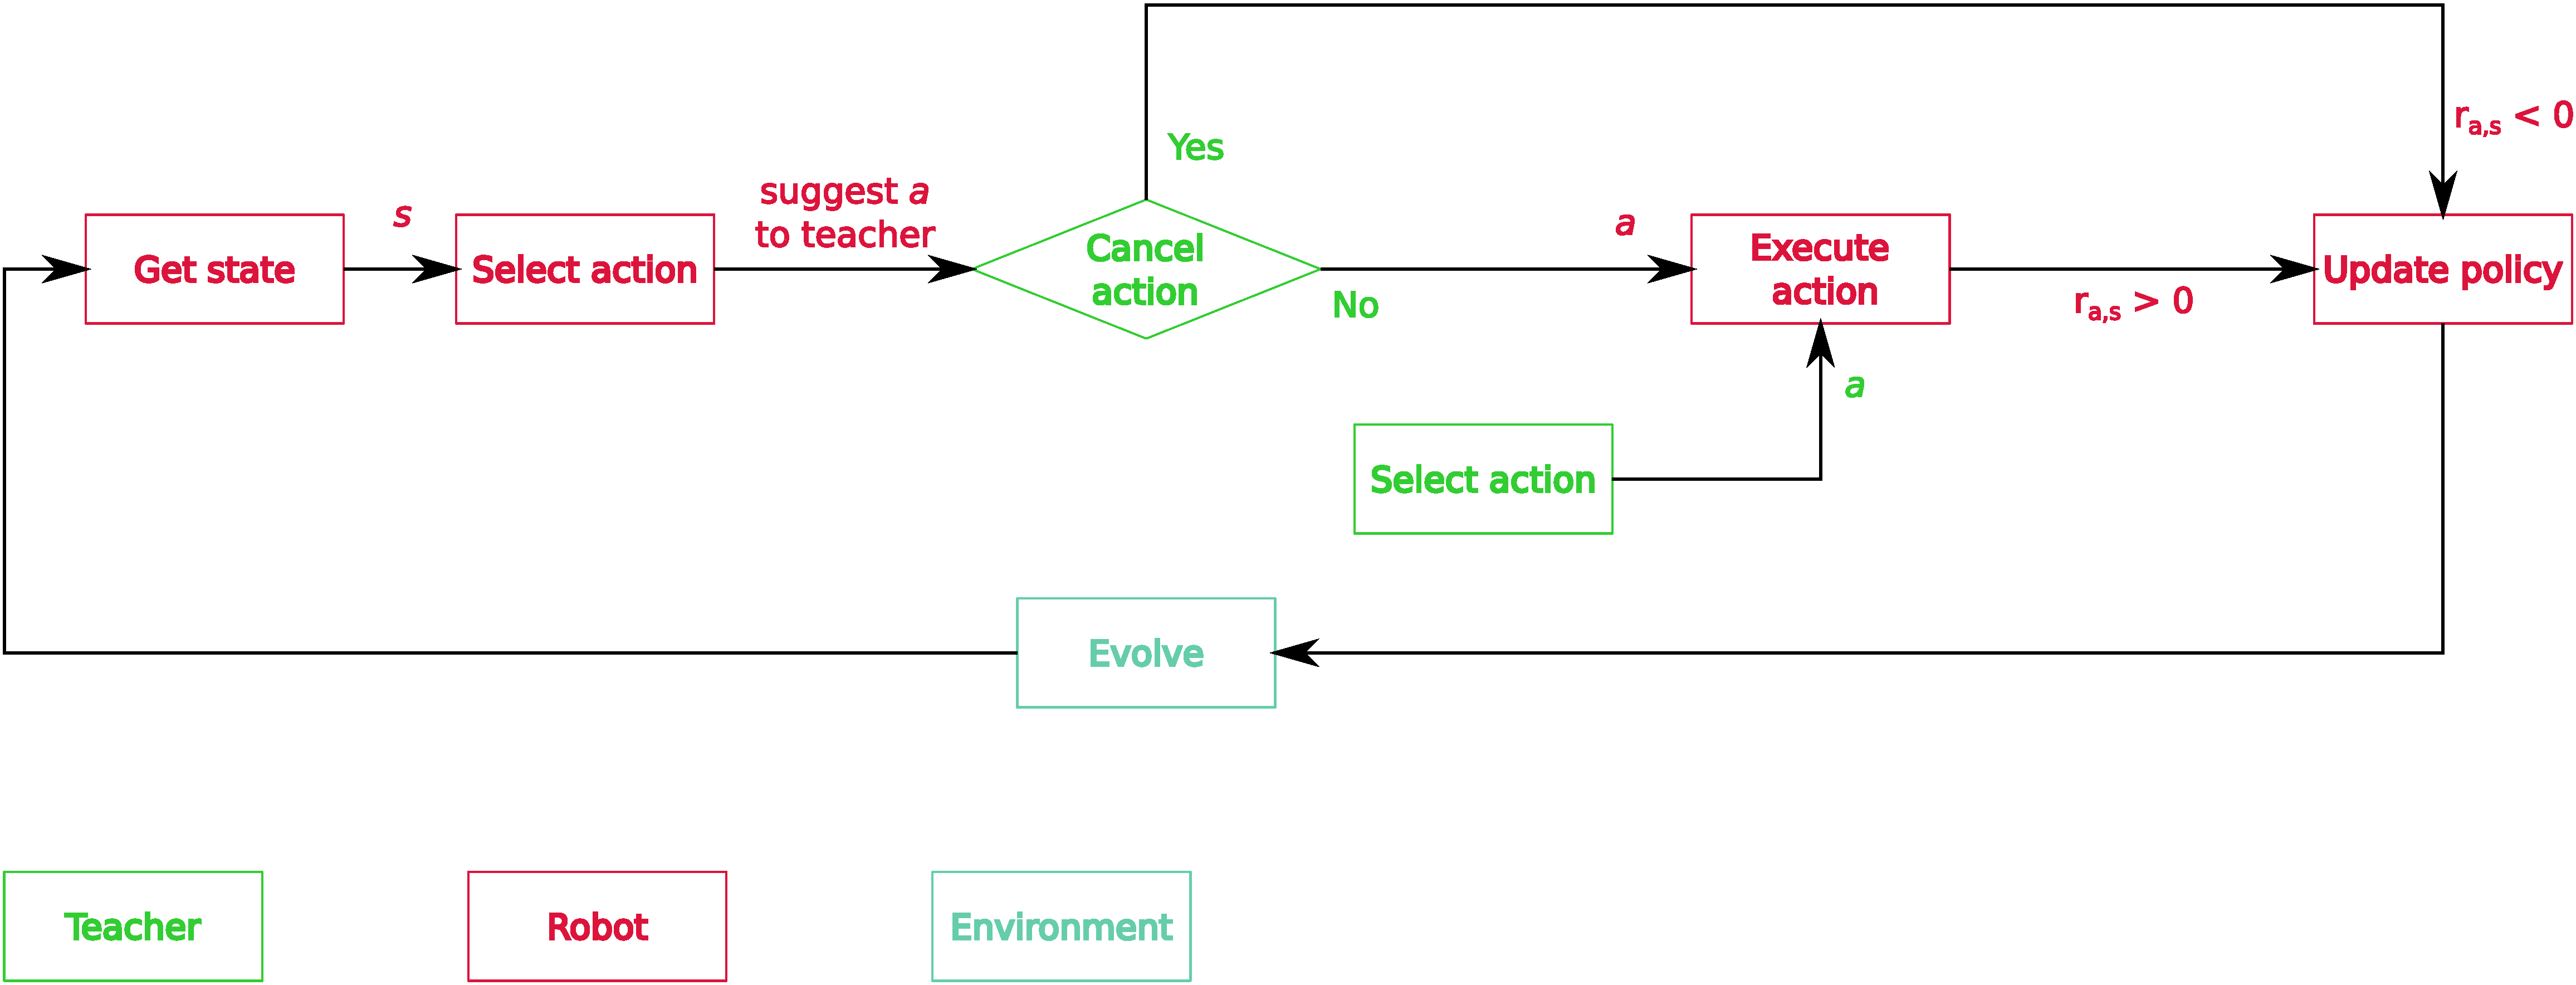
\includegraphics[width=1\linewidth]{flowchart.pdf}
	\centering
	\caption{Flowchart of the action selection loop between the agent and the teacher.}
	\label{fig:sparc_flowchart}
\end{figure}

This approach is comparable to predictive texting as seen on phone nowadays. The user can select the words proposed by the algorithms (or implicitly accept them by pressing the space bar) or write their own. The algorithm learns the user's preferences and habits and aims to suggest words more and more appropriate for the user. However, predictive texting aims mostly to correct users' errors and interact in a complex static environment. On the other hand, \gls{sparc} aims to replicate a teacher's action policy in continuous time, in a dynamic and interactive environment evolving both dependently and independently of the agent's actions.

Alternatively, \gls{sparc} can be seen as a way to provide proactivity to an agent. By observing interactions on longer time scales, such as an assistant robot at home, \gls{sparc} allows the robot to propose to help its user when the current state is similar to previous observation. This would compare to a passive case where each action executed by the robot has to be requested by the user or an autonomous robot interacting in the house without any transparency. By proposing actions to the teacher, the robot takes the initiative to support humans, possibly reminding its user something they forgot, while not imposing its presence. In human environments, executing actions (such as starting to play music, changing the lighting condition or cleaning the kitchen) without informing the surrounding humans could be perceived as rude or annoying if the timing is not right. On the other hand, this proactivity also needs to be kept in control as a robot proposing to help too often might be equally annoying.

\section{Goal}

\gls{sparc} aims to provide an interaction framework to teach robots an action policy possessing the following characteristics:
\begin{itemize}
	\item Be usable by people without expertise in computer science.
	\item Allow fast policy learning from \textit{in situ} guidance.
	\item Require few or no human input for the robot to act in the world.
	\item Constantly ensure an appropriate robot behaviour.
\end{itemize}

Figure~\ref{fig:concept} presents an idealistic comparison of the expected workload, performance and autonomy of four methods: autonomous learning (e.g. \gls{rl}; \citealt{sutton1998reinforcement}), feedback based teaching (e.g. TAMER; \citealt{knox2009interactively}), \gls{woz}~\citep{riek2012wizard} and \gls{sparc}. Unlike other learning methods, by following the principles presented in Section~\ref{sec:sparc_principles}, \gls{sparc} is expected to maintain a constant high performance even during early stages of learning. In later stages of the learning, the agent keeps improving its action policy, making its suggestions more accurate and allowing the auto-execution of actions to reduce the workload on the teacher.

\begin{figure}[ht]
	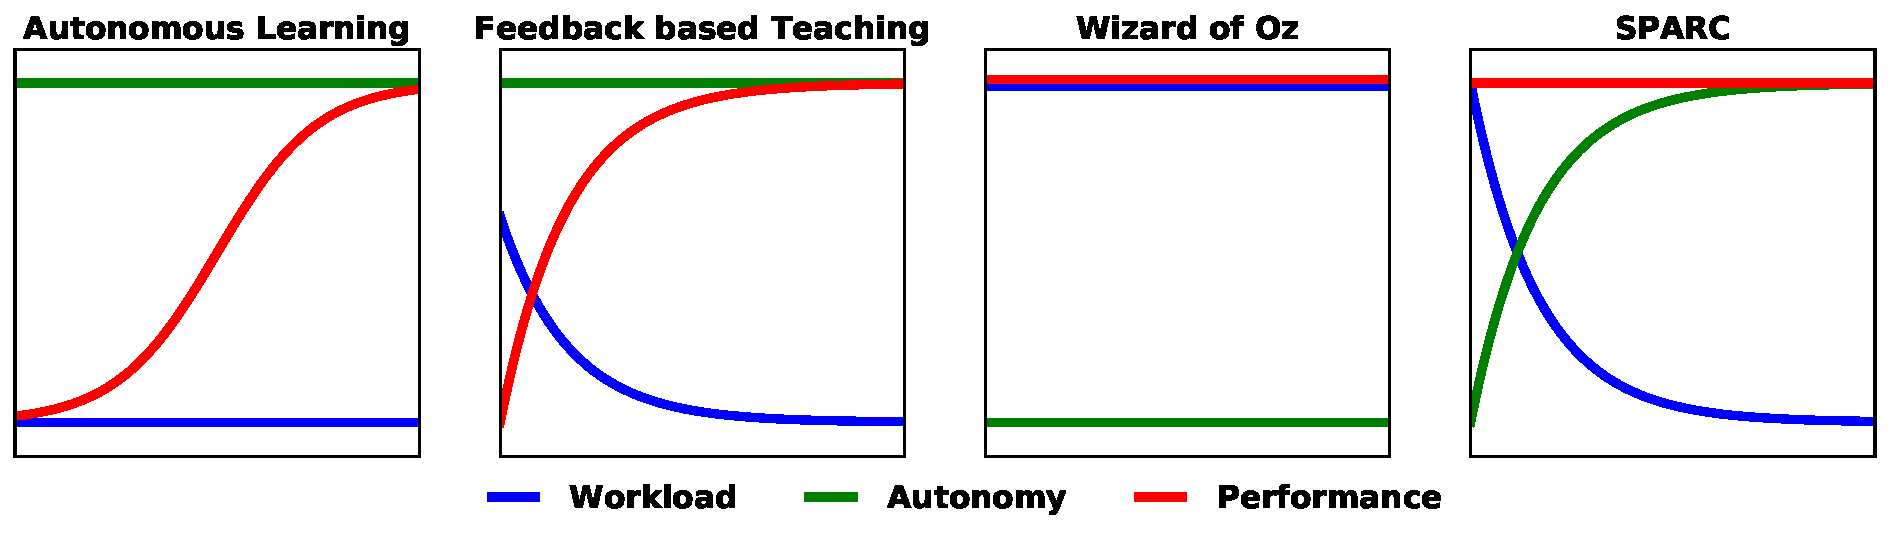
\includegraphics[width=1\linewidth]{concept.pdf}
	\centering
	\caption{Idealistic evolution of workload, performance, and autonomy over time for autonomous learning, feedback-based teaching, \gls{woz} and \gls{sparc} (arbitrary units).}
	\label{fig:concept}
\end{figure}
\ES{tenses}
Once the behaviour is deemed appropriate enough by the teacher, the agent is ready to be deployed to interact autonomously in the real world, if this outcome is desired. Alternatively, in contexts where a human expert still cannot be removed from the control loop, such as \gls{rat}, a supervisor could stay in control of the robot's actions by using the \gls{sa}. Similarly to the teaching phase, with this \gls{sa}, the robot would inform the supervisor of its actions and the human would only have to intervene in case of incorrect propositions. While still requiring attention from the supervisor, this reduction of human actions to control the robots would reduce the workload on the supervisor. Furthermore, as the supervisor would accumulate a better knowledge of the agent's behaviour, they could be especially careful in cases where the agent would be prone to making errors. And as the control of the agent would require less effort from the supervisor, they could focus more closely on the application interaction rather than the teaching one. 
%This approach is similar to safety drivers behind autonomous vehicles but with information about the car's intentions rather than solely observing the car's actions. 
%MAybe something on knowing critical parts of the interaction policy (Example DREAM only evaluation of performance)

\section{Implications}

\subsection{Relation with Time} \label{ssec:sparc_time}
Similarly to other \gls{iml} approaches, the requirement of a human in the action selection loop limits the time scale of interaction and this effect is an important consideration when applying \gls{sparc} to an interaction. With this type of \gls{iml}, three time scales are coexisting: the robot's, the teacher's and the interaction's. The robot has an internal clock running probably multiple times per second, sensing the world and deciding if an action should be proposed. The human teacher has to be able to cancel proposed actions before their executions, so they need to be provided with a `\gls{cw}' spanning more than one second to react to propositions. And finally, for some applications, actions are appropriate only during a short time, and if this amount of time (the \gls{vw}) is shorter than the \gls{cw}, action executed automatically would not be appropriate anymore, reducing the validity of \gls{sparc}.

Depending of the application, actions might have to be executed in a time critical environment (such as driving) or less critical ones (such as an assistant robot at home). While being easily applicable to slow interactions, \gls{sparc} could still be applied to these time critical ones. For instance, if applied to autonomous driving, \gls{sparc} could display to the driver the planned trajectory with augmented reality and let the driver correct this trajectory if not appropriate. However, more critical elements, such as emergency breaking, would probably have to be done with a much shorter correction window so the car can break in time. 

Additionally, the presence of this correction window reduces the rate of actions selection to 0.5 Hz or below, which might reduce the applicability of \gls{sparc} compared to other \gls{iml} methods. However, this limitation of application is the price to pay to ensure the appropriateness of actions, and this effect can be mitigated by using higher level actions or by focusing on applications less critical in term of time. 

Finally, the rate of selection of high level actions will be much lower than the rate of the robot's action selection loop. At a human level, actions will be executed at a rate of few actions per minutes, while the robot's processing runs at multiple hertz. This indicates that unlike classical \gls{rl} methods, in most of the steps, the robot should not select any action. When interacting with humans, the learning algorithm and the state representation needs to take into account these differences of time scales to ensure that the robot's behaviour is coherent and useful.

\subsection{Difference with \gls{lfd}}

\gls{sparc} is an \gls{ilfd} method (cf Section~\ref{ssec:back_ilfd}) and as it uses human demonstrations of policies to learn, it presents many similarities with non-interactive \gls{lfd} techniques (cf. Section~\ref{ssec:back_lfd}). However, most of the applications of \gls{lfd}~\citep{argall2009survey,billard2008robot} are focused on learning a manipulation skill in a mostly deterministic environment. \gls{lfd} has seldom been used to teach an action policy to interact with humans~\citep{liu2014train,sequeira2016discovering,munzer2017efficient} and never in an online fashion. Munzer et al. proposed an interactive planner that would learn offline the current user's preferences and desires, but two key differences exist between this approach and \gls{sparc}. The first one is the application domain. The learning planner is well suited to clearly defined environments (e.g. \gls{hrc}) where a similar task with clear steps has to be done multiple times. As such the learning can happen offline between the repetitions. \gls{sparc} is defined to be applicable to non-linear underspecified environments, with less constrained tasks, where the learning should happen online. Secondly, using a threshold, Munzer et al. define actions with low risk which are executed (and can be cancelled during the execution) and actions with higher risk which have to be validated first by the human. \gls{sparc} does not make this distinction, but proposes both types of actions to the teacher and will start executing them if no feedback is received. This removes the  need for the human to explicitly approve correct proposed actions while ensuring that the human can cancel incorrect actions before their execution. This principle aims at reducing the number of required interventions from the human to teach and interact with the robot compared to methods such as the one presented by Munzer et al. 

%Additionally, \gls{sparc} differs from Active Leaning (cf. Section~\ref{ssec:back_active}) by the fact that the agent cannot decide which sample will be evaluated by the teacher. As the robot interacts with humans, the datapoints provided to the teacher for labelling emerge from the interaction, and cannot be selected at will. 
    
%\section{Implications}

%The principles described in section~\ref{sec:sparc_principles} have also implications on the interactions between the teacher and the agent and between the agent and the environment. As the teacher has the power evaluate the actions proposed by the agent before their execution, it actually evaluates the intentions of the agent rather than its behaviour. This difference is key as traditional \gls{iml} approaches only evaluate the actions a posteriori by their effects. This implication is fundamental in \gls{hri} as a robot executing non appropriate actions when interacting with humans should not be deployed (cf. first principle in Section~\ref{ssec:back_constraints}) and asing the evaluation of the teacher on the intention rather than waiting for the action's outcome gives the opportunity to the teacher to preempt incorrect actions preventing the execution of undesired behaviours. The agent learns to avoid actions with expected negative impact without having to face the results of the execution of these undesired actions.

%Most importantly, the control given to the teacher on the agent's actions ensures that every action executed by the learner in the world has been either actively or passively validated by the teacher. This implies that each action executed can be assumed to be appropriate to the current state, potentially simplifying the learning algorithm.

\subsection{Interaction with Learning Algorithms}

The principles of \gls{sparc} define it at the crossroads between \gls{sl} and \gls{rl}. \gls{sparc} can be used in two ways: either to reproduce a teacher's policy in a supervised fashion or to help an agent discovering a useful action policy by using the teacher to bias the exploration, limiting the errors and only interacting in desired parts of the environment.

As such, \gls{sparc} only defines an interaction framework between a teacher and a learner and is agnostic to the learning mechanism: it can be combined with any algorithms used in \gls{sl} or \gls{rl}. This research presented in this thesis explored combinations with three types of algorithms: supervised learning using a feed-forward neural network (Chapter~\ref{chap:woz}), reinforcement learning (Chapter~\ref{chap:control}), and supervised learning using an instance based algorithm (Chapter~\ref{chap:tutoring}). However \gls{sparc} could be combined with a wide range of other algorithms or techniques such as planning.


Similarly to Inverse Reinforcement Learning~\citep{abbeel2004apprenticeship} or other techniques combining \gls{rl} and \gls{lfd}~\citep{billard2008robot}, if used with a reward function, \gls{sparc} could go beyond the demonstrated action policy and achieve a performance higher than the demonstration. However this aspect has not been evaluated in this work, but is discussed in Section~\ref{sec:disc_beyond}.

\section{Summary}
    
This chapter introduced the \acrfull{sparc}, a novel interaction framework to teach agents an action policy. This approach is suited to teach a robot to interact with humans as it validates the principles defined in Section~\ref{ssec:back_constraints} (appropriateness of action, adaptivity and autonomy). \gls{sparc} starts in a similar fashion than \gls{woz}: the teacher selects actions at any time to be executed by the robot. Then, using a learning algorithm, the agent starts to propose actions back to the teacher who can let them be executed after a short time or cancel them if not appropriate. This mechanism combining selections, suggestions and evaluations of actions ensures the appropriateness of the policy as a human expert could have preempted any inappropriate action before their execution. This additionally provides the adaptivity as the teacher can extend the robot behaviour beyond the current action policy. Finally, the learning algorithm associated with the auto-executions of actions intends to decrease the human workload once the robot starts to learn; and, when an acceptable action policy is reached, the robot is ready to be deployed to interact autonomously if this outcome is desired.
